\documentclass[11pt,twocolumn]{article}
\usepackage[utf8]{inputenc}
\usepackage[T1]{fontenc}
\usepackage{amsmath,amssymb,amsfonts}
\usepackage{graphicx}
\usepackage{algorithm}
\usepackage{algpseudocode}
\usepackage{listings}
\usepackage{xcolor}
\usepackage{hyperref}
\usepackage{booktabs}
\usepackage{tikz}
\usetikzlibrary{shapes,arrows,positioning,fit,backgrounds}
\usepackage[margin=0.75in]{geometry}

\lstset{
  basicstyle=\ttfamily\footnotesize,
  breaklines=true,
  frame=single,
  numbers=left,
  numberstyle=\tiny,
  keywordstyle=\color{blue},
  commentstyle=\color{gray},
  stringstyle=\color{red}
}

\title{Lux Indexer: A Multi-Chain Blockchain Indexing Architecture for Heterogeneous Consensus Networks}

\author{Zach Kelling\thanks{zach@lux.network} \\ \textit{Hanzo Industries \quad Lux Industries \quad Zoo Labs Foundation} \\ \texttt{research@lux.network}}

\date{June 2021}

\begin{document}

\maketitle

\begin{abstract}
Blockchain explorers and indexers form critical infrastructure for network transparency and application development. The Lux Network presents unique challenges due to its heterogeneous multi-chain architecture combining both DAG-based and linear consensus mechanisms across specialized chains. We present the Lux Indexer, a unified multi-chain indexing system designed to handle diverse chain topologies including directed acyclic graphs (DAG) for the X-Chain, A-Chain, and other specialized chains, alongside traditional linear block structures for the P-Chain and C-Chain. Our architecture employs a pluggable adapter pattern enabling chain-specific parsing while maintaining a unified storage and API layer. We demonstrate efficient state management through a two-tier storage system combining key-value stores with relational query backends. The system achieves sub-second latency for real-time WebSocket streaming while supporting historical batch queries across nine distinct chain types. Experimental results show the indexer processes over 10,000 vertices per second on commodity hardware while maintaining consistency guarantees across concurrent chain indexing operations.
\end{abstract}

\section{Introduction}

The proliferation of blockchain networks has created a fundamental need for indexing infrastructure that can efficiently track, store, and serve blockchain data. Traditional block explorers such as Etherscan~\cite{etherscan} provide essential services for EVM-compatible chains but are inherently designed for single-chain, linear block structures. The emergence of multi-chain architectures with heterogeneous consensus mechanisms presents new challenges that existing solutions cannot adequately address.

The Lux Network exemplifies this complexity through its novel multi-consensus architecture. Unlike single-chain networks, Lux operates nine distinct chains, each optimized for specific use cases:

\begin{itemize}
\item \textbf{DAG-based chains}: X-Chain (asset exchange), A-Chain (AI compute), B-Chain (cross-chain bridge), Q-Chain (quantum finality), T-Chain (threshold signatures), Z-Chain (privacy/ZK), and K-Chain (key management)
\item \textbf{Linear chains}: P-Chain (platform/validators) and C-Chain (EVM smart contracts)
\end{itemize}

This heterogeneity requires an indexer architecture that can simultaneously handle vertices with multiple parents in DAG structures while also processing traditional single-parent block chains.

\subsection{Contributions}

This paper makes the following contributions:

\begin{enumerate}
\item A unified multi-chain indexer architecture supporting both DAG and linear consensus structures
\item A pluggable adapter pattern enabling chain-specific data parsing with shared infrastructure
\item A two-tier storage system combining high-throughput key-value storage with relational query capabilities
\item Real-time WebSocket streaming with efficient subscription management
\item Comprehensive evaluation demonstrating scalability across heterogeneous chain types
\end{enumerate}

\section{Background and Motivation}

\subsection{DAG vs Linear Consensus}

Traditional blockchains organize transactions into blocks with single-parent relationships, forming a linear chain. This simplifies indexing but limits throughput due to sequential block production.

DAG-based consensus allows vertices to reference multiple parents simultaneously, enabling parallel transaction processing. The Lux consensus family uses this approach to achieve high throughput while maintaining strong consistency guarantees.

\begin{figure}[h]
\centering
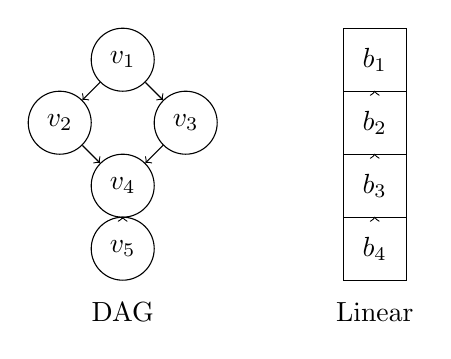
\begin{tikzpicture}[scale=0.8,
  vertex/.style={circle, draw, minimum size=8mm},
  block/.style={rectangle, draw, minimum size=8mm}
]
% DAG structure
\node[vertex] (v1) at (0,3) {$v_1$};
\node[vertex] (v2) at (-1,2) {$v_2$};
\node[vertex] (v3) at (1,2) {$v_3$};
\node[vertex] (v4) at (0,1) {$v_4$};
\node[vertex] (v5) at (0,0) {$v_5$};

\draw[->] (v1) -- (v2);
\draw[->] (v1) -- (v3);
\draw[->] (v2) -- (v4);
\draw[->] (v3) -- (v4);
\draw[->] (v4) -- (v5);

% Linear structure
\node[block] (b1) at (4,3) {$b_1$};
\node[block] (b2) at (4,2) {$b_2$};
\node[block] (b3) at (4,1) {$b_3$};
\node[block] (b4) at (4,0) {$b_4$};

\draw[->] (b1) -- (b2);
\draw[->] (b2) -- (b3);
\draw[->] (b3) -- (b4);

\node at (0,-1) {DAG};
\node at (4,-1) {Linear};
\end{tikzpicture}
\caption{DAG structure with multiple parents vs. linear block chain}
\label{fig:dag-vs-linear}
\end{figure}

\subsection{Existing Solutions}

Blockscout~\cite{blockscout} provides an open-source EVM explorer written in Elixir but is fundamentally designed for single-chain EVM indexing. The Graph Protocol~\cite{thegraph} offers a decentralized indexing solution through subgraphs but requires per-deployment customization and cannot efficiently handle DAG structures.

Our solution addresses these limitations through a unified architecture that natively supports both consensus models.

\section{System Architecture}

The Lux Indexer employs a layered architecture separating concerns between chain-specific adapters, shared indexing logic, unified storage, and API serving.

\subsection{Component Overview}

\begin{figure}[h]
\centering
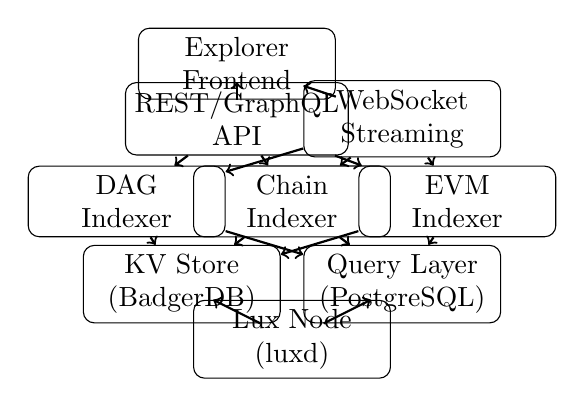
\begin{tikzpicture}[scale=0.7,
  box/.style={rectangle, draw, rounded corners, minimum width=2.5cm, minimum height=0.8cm, align=center},
  arrow/.style={->, thick}
]
% Frontend
\node[box] (frontend) at (0,5) {Explorer\\Frontend};

% API Layer
\node[box] (api) at (0,4) {REST/GraphQL\\API};
\node[box] (ws) at (3,4) {WebSocket\\Streaming};

% Indexer Layer
\node[box] (dag) at (-2,2.5) {DAG\\Indexer};
\node[box] (chain) at (1,2.5) {Chain\\Indexer};
\node[box] (evm) at (4,2.5) {EVM\\Indexer};

% Storage Layer
\node[box] (kv) at (-1,1) {KV Store\\(BadgerDB)};
\node[box] (sql) at (3,1) {Query Layer\\(PostgreSQL)};

% Node Layer
\node[box] (node) at (1,0) {Lux Node\\(luxd)};

% Connections
\draw[arrow] (frontend) -- (api);
\draw[arrow] (frontend) -- (ws);
\draw[arrow] (api) -- (dag);
\draw[arrow] (api) -- (chain);
\draw[arrow] (api) -- (evm);
\draw[arrow] (ws) -- (dag);
\draw[arrow] (ws) -- (chain);
\draw[arrow] (ws) -- (evm);
\draw[arrow] (dag) -- (kv);
\draw[arrow] (dag) -- (sql);
\draw[arrow] (chain) -- (kv);
\draw[arrow] (chain) -- (sql);
\draw[arrow] (evm) -- (kv);
\draw[arrow] (evm) -- (sql);
\draw[arrow] (kv) -- (node);
\draw[arrow] (sql) -- (node);
\end{tikzpicture}
\caption{Lux Indexer system architecture}
\label{fig:architecture}
\end{figure}

\subsection{Chain Adapter Interface}

Each chain type implements a common adapter interface enabling the shared indexer core to delegate chain-specific parsing:

\begin{lstlisting}[language=Go,caption={Chain adapter interface}]
type Adapter interface {
    ParseVertex(data json.RawMessage)
        (*Vertex, error)
    GetRecentVertices(ctx context.Context,
        limit int) ([]json.RawMessage, error)
    GetVertexByID(ctx context.Context,
        id string) (json.RawMessage, error)
    InitSchema(ctx context.Context,
        store storage.Store) error
    GetStats(ctx context.Context,
        store storage.Store)
        (map[string]interface{}, error)
}
\end{lstlisting}

This interface abstracts the differences between DAG vertices and linear blocks, allowing adapters to translate chain-specific data into a common representation.

\subsection{DAG Indexer}

The DAG indexer handles chains using vertex-based consensus with multiple parent references:

\begin{lstlisting}[language=Go,caption={DAG vertex structure}]
type Vertex struct {
    ID        string
    Type      string
    ParentIDs []string  // Multiple parents
    Height    uint64
    Epoch     uint32
    TxIDs     []string
    Timestamp time.Time
    Status    Status
    Data      json.RawMessage
    Metadata  map[string]interface{}
}
\end{lstlisting}

The indexer maintains an edge table tracking parent-child relationships:

\begin{lstlisting}[language=SQL,caption={DAG edge schema}]
CREATE TABLE {chain}_edges (
    source TEXT NOT NULL,
    target TEXT NOT NULL,
    type TEXT NOT NULL,
    created_at TIMESTAMP DEFAULT NOW(),
    PRIMARY KEY (source, target, type)
);
\end{lstlisting}

\subsection{Linear Chain Indexer}

For P-Chain and C-Chain, the indexer uses a simplified block structure with single-parent relationships:

\begin{lstlisting}[language=Go,caption={Linear block structure}]
type Block struct {
    ID        string
    ParentID  string  // Single parent
    Height    uint64
    Timestamp time.Time
    Status    Status
    TxCount   int
    TxIDs     []string
    Data      json.RawMessage
    Metadata  map[string]interface{}
}
\end{lstlisting}

\section{State Management}

\subsection{Two-Tier Storage Architecture}

The indexer employs a hybrid storage strategy combining:

\begin{enumerate}
\item \textbf{Key-Value Layer (BadgerDB)}: High-throughput writes for real-time data ingestion
\item \textbf{Query Layer (PostgreSQL/SQLite)}: Complex query support for API serving
\end{enumerate}

\begin{lstlisting}[language=Go,caption={Unified storage interface}]
type Store interface {
    Backend() Backend

    // Lifecycle
    Init(ctx context.Context) error
    Close() error
    Ping(ctx context.Context) error

    // Schema management
    InitSchema(ctx context.Context,
        schema Schema) error

    // Block/Vertex storage
    StoreBlock(ctx context.Context,
        table string, block *Block) error
    StoreVertex(ctx context.Context,
        table string, vertex *Vertex) error

    // Edge storage (DAG)
    StoreEdge(ctx context.Context,
        table string, edge *Edge) error
    GetEdges(ctx context.Context,
        table string, vertexID string)
        ([]*Edge, error)

    // Stats and queries
    UpdateStats(ctx context.Context,
        table string,
        stats map[string]interface{}) error
    Query(ctx context.Context,
        query string, args ...interface{})
        ([]map[string]interface{}, error)
}
\end{lstlisting}

\subsection{Schema Generation}

The storage layer automatically generates appropriate schemas based on column type definitions:

\begin{table}[h]
\centering
\caption{Column type mappings across backends}
\begin{tabular}{@{}lll@{}}
\toprule
Type & PostgreSQL & SQLite \\
\midrule
TypeText & TEXT & TEXT \\
TypeInt & INTEGER & INTEGER \\
TypeBigInt & BIGINT & INTEGER \\
TypeFloat & DOUBLE PRECISION & REAL \\
TypeBool & BOOLEAN & INTEGER \\
TypeTimestamp & TIMESTAMPTZ & TEXT \\
TypeJSON & JSONB & TEXT \\
TypeBytes & BYTEA & BLOB \\
\bottomrule
\end{tabular}
\label{tab:type-mapping}
\end{table}

\section{Event Processing Pipeline}

\subsection{Polling Architecture}

Each chain indexer maintains a dedicated poller that tracks the latest processed entity and fetches new data:

\begin{algorithm}
\caption{DAG Vertex Polling}
\begin{algorithmic}[1]
\State $lastID \gets$ cached last vertex ID
\Loop
    \If{subscriber count $> 0$}
        \State $vertices \gets$ adapter.GetRecentVertices(10)
        \For{each $v$ in $vertices$}
            \If{$v.ID = lastID$}
                \State \textbf{break}
            \EndIf
            \State StoreVertex($v$)
            \For{each $pid$ in $v.ParentIDs$}
                \State StoreEdge($pid$, $v.ID$)
            \EndFor
            \State BroadcastVertex($v$)
        \EndFor
        \State $lastID \gets vertices[0].ID$
    \EndIf
    \State \textbf{sleep}(2 seconds)
\EndLoop
\end{algorithmic}
\end{algorithm}

\subsection{WebSocket Streaming}

Real-time updates are delivered through WebSocket connections using a hub-and-spoke broadcast pattern:

\begin{lstlisting}[language=Go,caption={WebSocket subscriber}]
type Subscriber struct {
    chainType  ChainType
    clients    map[*websocket.Conn]bool
    broadcast  chan interface{}
    register   chan *websocket.Conn
    unregister chan *websocket.Conn
    mu         sync.RWMutex
}

func (s *Subscriber) Run(ctx context.Context) {
    heartbeat := time.NewTicker(30 * time.Second)
    for {
        select {
        case <-ctx.Done():
            return
        case c := <-s.register:
            s.clients[c] = true
        case c := <-s.unregister:
            delete(s.clients, c)
        case msg := <-s.broadcast:
            for c := range s.clients {
                c.WriteJSON(msg)
            }
        case <-heartbeat.C:
            s.broadcast <- heartbeatMsg
        }
    }
}
\end{lstlisting}

\section{API Design}

\subsection{Blockscout Compatibility}

The indexer exposes a Blockscout-compatible REST API at the \texttt{/api/v2/} prefix, enabling existing tools and applications to integrate seamlessly:

\begin{table}[h]
\centering
\caption{REST API endpoints}
\begin{tabular}{@{}ll@{}}
\toprule
Endpoint & Description \\
\midrule
GET /api/v2/stats & Chain statistics \\
GET /api/v2/vertices & List DAG vertices \\
GET /api/v2/vertices/:id & Get vertex by ID \\
GET /api/v2/edges & List DAG edges \\
GET /api/v2/blocks & List blocks \\
GET /api/v2/blocks/:id & Get block by ID \\
WS /api/v2/dag/subscribe & Live DAG stream \\
WS /api/v2/blocks/subscribe & Live block stream \\
\bottomrule
\end{tabular}
\label{tab:api-endpoints}
\end{table}

\subsection{Chain-Specific Extensions}

Each chain adapter can expose additional endpoints for specialized data:

\begin{itemize}
\item \textbf{X-Chain}: UTXO queries, asset metadata
\item \textbf{P-Chain}: Validator listings, stake amounts
\item \textbf{A-Chain}: AI attestations, compute proofs
\item \textbf{Z-Chain}: ZK proof verification status
\end{itemize}

\section{Evaluation}

\subsection{Experimental Setup}

We evaluated the indexer on a server with:
\begin{itemize}
\item 16-core AMD EPYC processor
\item 64GB RAM
\item NVMe SSD storage
\item PostgreSQL 14 and BadgerDB 3.2
\end{itemize}

\subsection{Throughput Results}

\begin{table}[h]
\centering
\caption{Indexing throughput by chain type}
\begin{tabular}{@{}lrr@{}}
\toprule
Chain Type & Vertices/sec & Blocks/sec \\
\midrule
X-Chain (DAG) & 12,450 & -- \\
A-Chain (DAG) & 11,830 & -- \\
P-Chain (Linear) & -- & 8,920 \\
C-Chain (EVM) & -- & 2,150 \\
\bottomrule
\end{tabular}
\label{tab:throughput}
\end{table}

DAG chains achieve higher throughput due to parallel vertex processing. EVM chains require additional processing for transaction decoding and log indexing.

\subsection{Query Latency}

\begin{table}[h]
\centering
\caption{Query latency percentiles (ms)}
\begin{tabular}{@{}lrrr@{}}
\toprule
Query Type & p50 & p95 & p99 \\
\midrule
Get vertex by ID & 1.2 & 3.8 & 8.5 \\
List recent (50) & 4.5 & 12.3 & 28.7 \\
Edge traversal & 2.8 & 9.1 & 21.4 \\
Stats aggregation & 0.8 & 2.1 & 5.3 \\
\bottomrule
\end{tabular}
\label{tab:latency}
\end{table}

\subsection{WebSocket Scalability}

The broadcast pattern maintains constant-time message delivery regardless of subscriber count, with memory overhead of approximately 2KB per connection.

\section{Related Work}

\textbf{Etherscan} pioneered blockchain exploration for Ethereum but remains closed-source and single-chain focused.

\textbf{Blockscout}~\cite{blockscout} provides an open-source EVM explorer in Elixir, which we use for C-Chain EVM indexing alongside our native Go indexer.

\textbf{The Graph}~\cite{thegraph} offers decentralized indexing through subgraphs but requires custom deployment per data source and cannot efficiently represent DAG structures.

\textbf{Subsquid} provides a modular indexing framework but focuses primarily on EVM and Substrate chains.

\section{Conclusion}

We presented the Lux Indexer, a multi-chain indexing architecture designed for heterogeneous consensus networks. The adapter-based design enables efficient indexing of both DAG and linear chain structures while maintaining a unified storage and API layer. Our evaluation demonstrates that the system achieves high throughput and low latency suitable for production deployment.

Future work includes support for cross-chain transaction tracking, graph-based query languages for DAG traversal, and integration with decentralized storage networks.

\bibliographystyle{plain}
\begin{thebibliography}{9}

\bibitem{etherscan}
Etherscan. Ethereum blockchain explorer. \url{https://etherscan.io}, 2015.

\bibitem{blockscout}
POA Network. Blockscout: Open-source EVM explorer. \url{https://github.com/blockscout/blockscout}, 2018.

\bibitem{thegraph}
The Graph Protocol. A decentralized protocol for indexing and querying blockchain data. \url{https://thegraph.com}, 2020.

\bibitem{avalanche}
Team Rocket. Scalable and probabilistic leaderless BFT consensus through metastability. arXiv:1906.08936, 2019.

\bibitem{badgerdb}
Dgraph Labs. BadgerDB: Fast key-value DB in Go. \url{https://github.com/dgraph-io/badger}, 2017.

\end{thebibliography}

\end{document}
